\title{Study Guide for Midterm}
\author{Dr. Jordan Hanson - Whittier College Dept. of Physics and Astronomy}
\date{\today}
\documentclass[10pt]{article}
\usepackage[a4paper, total={18cm, 27cm}]{geometry}
\usepackage{outlines}
\usepackage{graphicx}
\begin{document}
\maketitle

\section{Chapter 1 - Introductory Concepts}
\begin{figure}[ht]
\centering
\includegraphics[width=0.75\textwidth]{timingExample1.pdf}
\caption{\label{fig:timing1} A timing diagram including a clock signal (CLK), a 4-bit parallel data stream (D0-D3), and enable/disable signals (EN/$\sim$EN).}
\end{figure}
\begin{enumerate}
\item Consider Fig. \ref{fig:timing1}. (a) If the clock frequency is 10 MHz, what is the period?  (b) What is the length of time represented in the waveform? (c) What is the length of the pulse in channel $D0$? \\ \vspace{2.5cm}
\item (a) What is the bit sequence represented by $D3$? (b) If $D0$ is a periodic signal, what is the duty cycle? \\ \vspace{1cm}
\item (a) Imagine that the four $D_i$ signals enter an AND gate, along with the EN signal.  Draw the resulting timing diagram. (b) Imagine that the four $D_i$ signals enter an AND gate, along with the $\sim$EN signal.  Draw the resulting timing diagram. \\ \vspace{3cm}
\item Suppose $D_i$ represents parallel data.  Each line gives 16 bits, and the clock frequency is 10 MHz.  (a) How many total bits are being sent across the $D_i$, and how long does it take?  What is the ratio of total bits to time?  (b) What would this time be if the data was transferred \textit{serially}, instead of in \textit{parallel}? \\ \vspace{2cm}
\end{enumerate}

\section{Chapter 2 - Number Systems, Operations, and Codes}

\begin{enumerate}
\item Convert the following numbers to binary: (a) 33 (b) 65 (c) 129. (d) What does each number have in common? (e) Sketch a short python script to convert a decimal number to binary, and return the result. \\ \vspace{3cm}
\item Represent the following numbers in 8-bit binary: (a) -31 (b) -15 (c) -7.  (d) Show that each number, when added to its opposite is zero, in binary.  (e) Did you know that the \textit{shift} operators in C and Python can act as binary multipliers?  For example \verb+2 << 1+ results in 4.  Why? Because the code is saying $0010 \rightarrow 0100$. What is the result of the following codes in Python? 
\begin{verbatim}
j = 1
for i in range(0,5):
	print(j << i)	
\end{verbatim}
\vspace{3cm}
\item What is the largest number that can be represented in binary with (a) $n = 4$ (b) $n = 8$ bits, if one bit must be used as a sign bit? \\ \vspace{2cm}
\item Convert the following numbers to binary: (a) 0xFE (b) 0x7F (c) 0x3F. \\ \vspace{2cm}
\item Convert to hexadecimal: 1000100001000100 \\ \vspace{2cm}
\item What is the following gray code sequence: 0011 0010 0111 0100 1110? \\ \vspace{2cm}
\end{enumerate}

\clearpage

\section{Chapter 3 - Logic Gates}
\begin{figure}[ht]
\centering
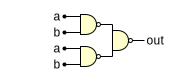
\includegraphics[width=0.3\textwidth]{gateExample1.pdf}
\includegraphics[width=0.3\textwidth]{gateExample2.pdf}
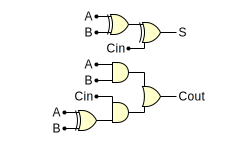
\includegraphics[width=0.3\textwidth]{gateExample3.pdf}
\caption{\label{fig:gates1} Examples of logic gate combinations.}
\end{figure}
\begin{enumerate}
\item Generate the truth tables for the gate diagrams in Fig. \ref{fig:gates1}. Pay attention to the domain.  \\ \vspace{3cm}
\item Identify the actions of the gate combinations in the previous problem from the truth tables.  (a) Fig. \ref{fig:gates1}, left:\rule{3cm}{0.1mm} (b) Fig. \ref{fig:gates1}, middle:\rule{3cm}{0.1mm} (c) Fig. \ref{fig:gates1}, right:\rule{3cm}{0.1mm}.
\item Suppose the signals in Fig. \ref{fig:timing2} are fed into the circuit in Fig. \ref{fig:gates1}, right.  Fill in the S and Cout signals in Fig. \ref{fig:timing2}.
\item Imagine a system for an electronic door lock which requires two electronic keys (two signals), S1 and S2.  The circuit has a red LED, a yellow LED, and a green LED.  The system unlocks when the output LOCK signal is LOW, caused by a LOW S1 and a LOW S2.  The red LED is activated when S1 and S2 are both HIGH.  The yellow LED is activated when S1 and S2 are different.  The green LED is activated when the system is unlocked.  \textit{By default, S1 and S2 are HIGH.} Draw the solution below.  \\ \vspace{4cm}
\end{enumerate}
\begin{figure}[hb]
\centering
\includegraphics[width=0.5\textwidth]{timingExample2.pdf}
\caption{\label{fig:timing2} An example timing diagram for Fig. \ref{fig:gates1}, right.  The shaded regions indicate ``don't care'' conditions, or times when the data is not relevant.}
\end{figure}

\section{Chapter 4 - Boolean Algebra and Logic Simplification}
\begin{figure}[ht]
\centering
\includegraphics[width=0.4\textwidth]{gateExample4.pdf}
\caption{\label{fig:gates2} A gate combination triggering a signal named ``record.''}
\end{figure}
\begin{enumerate}
\item Consider the circuit in Fig. \ref{fig:gates2}.  (a) Write a logic expression for \textit{Record}. (b) Simplify the expression to as minimal a form as possible. (c) Are any signals or gates unnecessary? \\ \vspace{3cm}
\item Consider again the logic expression that represents the circuit in Fig. \ref{fig:gates2}. (a) Write the corresponding domain-4 Karnaugh map.  (b) Use the Karnaugh map to produce the S-POS expression and truth table. \\ \vspace{3cm}
\end{enumerate}

\section{Chapter 5 - Combinatorial Logic Analysis}
\label{sec:comb}
\begin{figure}[ht]
\centering
\includegraphics[width=0.5\textwidth]{timingExample3.pdf}
\caption{\label{fig:timing3} Timing diagram for Sec. \ref{sec:comb}.}
\end{figure}
\begin{enumerate}
\item (a) Draw the circuit corresponding to the timing diagram in Fig. \ref{fig:timing3}.  (b) Create the Karnaugh map.  (c) Using the Karnaugh map, write the simplest expression for this logic function and re-draw the circuit.
\end{enumerate}

\end{document}